%%% The main file. It contains definitions of basic parameters and includes all other parts.

%% Settings for single-side (simplex) printing
% Margins: left 40mm, right 25mm, top and bottom 25mm
% (but beware, LaTeX adds 1in implicitly)
\documentclass[12pt,a4paper]{report}
\setlength\textwidth{145mm}
\setlength\textheight{247mm}
\setlength\oddsidemargin{15mm}
\setlength\evensidemargin{15mm}
\setlength\topmargin{0mm}
\setlength\headsep{0mm}
\setlength\headheight{0mm}
% \openright makes the following text appear on a right-hand page
\let\openright=\clearpage

%% Settings for two-sided (duplex) printing
% \documentclass[12pt,a4paper,twoside,openright]{report}
% \setlength\textwidth{145mm}
% \setlength\textheight{247mm}
% \setlength\oddsidemargin{14.2mm}
% \setlength\evensidemargin{0mm}
% \setlength\topmargin{0mm}
% \setlength\headsep{0mm}
% \setlength\headheight{0mm}
% \let\openright=\cleardoublepage

%% Generate PDF/A-2u
\usepackage[a-2u]{pdfx}

%% Character encoding: usually latin2, cp1250 or utf8:
\usepackage[utf8]{inputenc}

%% Prefer Latin Modern fonts
\usepackage{lmodern}

%% Further useful packages (included in most LaTeX distributions)
\usepackage{amsmath}        % extensions for typesetting of math
\usepackage{amsfonts}       % math fonts
\usepackage{amsthm}         % theorems, definitions, etc.
\usepackage{bm}             % boldface symbols (\bm)
\usepackage{graphicx}       % embedding of pictures
\usepackage{fancyvrb}       % improved verbatim environment
\usepackage{natbib}         % citation style AUTHOR (YEAR), or AUTHOR [NUMBER]
\usepackage[nottoc]{tocbibind} % makes sure that bibliography and the lists
			    % of figures/tables are included in the table
			    % of contents
\usepackage{dcolumn}        % improved alignment of table columns
\usepackage{booktabs}       % improved horizontal lines in tables
\usepackage{paralist}       % improved enumerate and itemize
\usepackage{xcolor}         % typesetting in color
\usepackage{url}
\usepackage{verbatim}
%%% Basic information on the thesis

\usepackage{acronym}
\usepackage{makecell}
\usepackage{listings}
\usepackage{enumitem}
\usepackage{bbding}
\newcommand\short{}

\newcommand{\emptyline}{\vspace{\baselineskip}}

\newcommand{\multilinebox}[1]{
    \begin{center}
        \framebox{
            \begin{minipage}{0.9\textwidth}
                #1
            \end{minipage}
        }
    \end{center}
}

\newcommand{\numb}[1]{
    \arabic{#1}
    \stepcounter{#1}
}

% Thesis title in English (exactly as in the formal assignment)
\def\ThesisTitle{Declarative Web Automation Toolkit}

% Author of the thesis
\def\ThesisAuthor{Jindřich Bär}

% Year when the thesis is submitted
\def\YearSubmitted{2022}

% Name of the department or institute where the work was officially assigned
% (according to the Organizational Structure of MFF UK in English,
% or a full name of a department outside MFF)
\def\Department{Department of Software Engineering}

% Is it a department (katedra), or an institute (ústav)?
\def\DeptType{Department}

% Thesis supervisor: name, surname, and titles
\def\Supervisor{RNDr. Jakub Klímek, Ph.D.}

% Supervisor's department (again according to Organizational structure of MFF)
\def\SupervisorsDepartment{Department of Software Engineering}

% Study programme and specialization
\def\StudyProgramme{Computer Science}
\def\StudyBranch{Databases and Web}

% An optional dedication: you can thank whomever you wish (your supervisor,
% consultant, a person who lent the software, etc.)
\def\Dedication{%
Dedication.
}

% Abstract (recommended length around 80-200 words; this is not a copy of your thesis assignment!)
\def\Abstract{%
Abstract.
}

% 3 to 5 keywords (recommended), each enclosed in curly braces
\def\Keywords{%
{web} {automation} {scraper} {crawler} {declarative programming}
}

%% The hyperref package for clickable links in PDF and also for storing
%% metadata to PDF (including the table of contents).
%% Most settings are pre-set by the pdfx package.
\hypersetup{unicode}
\hypersetup{breaklinks=true}

% Definitions of macros (see description inside)
%%% This file contains definitions of various useful macros and environments %%%
%%% Please add more macros here instead of cluttering other files with them. %%%

%%% Minor tweaks of style

% These macros employ a little dirty trick to convince LaTeX to typeset
% chapter headings sanely, without lots of empty space above them.
% Feel free to ignore.
\makeatletter
\def\@makechapterhead#1{
  {\parindent \z@ \raggedright \normalfont
   \Huge\bfseries \thechapter. #1
   \par\nobreak
   \vskip 20\p@
}}
\def\@makeschapterhead#1{
  {\parindent \z@ \raggedright \normalfont
   \Huge\bfseries #1
   \par\nobreak
   \vskip 20\p@
}}
\makeatother

% This macro defines a chapter, which is not numbered, but is included
% in the table of contents.
\def\chapwithtoc#1{
\chapter*{#1}
\addcontentsline{toc}{chapter}{#1}
}

% Draw black "slugs" whenever a line overflows, so that we can spot it easily.
\overfullrule=1mm

%%% Macros for definitions, theorems, claims, examples, ... (requires amsthm package)

\theoremstyle{plain}
\newtheorem{thm}{Theorem}
\newtheorem{lemma}[thm]{Lemma}
\newtheorem{claim}[thm]{Claim}

\theoremstyle{plain}
\newtheorem{defn}{Definition}

\theoremstyle{remark}
\newtheorem*{cor}{Corollary}
\newtheorem*{rem}{Remark}
\newtheorem*{example}{Example}

%%% An environment for proofs

\newenvironment{myproof}{
  \par\medskip\noindent
  \textit{Proof}.
}{
\newline
\rightline{$\qedsymbol$}
}

%%% An environment for typesetting of program code and input/output
%%% of programs. (Requires the fancyvrb package -- fancy verbatim.)

\DefineVerbatimEnvironment{code}{Verbatim}{fontsize=\small, frame=single}

%%% The field of all real and natural numbers
\newcommand{\R}{\mathbb{R}}
\newcommand{\N}{\mathbb{N}}

%%% Useful operators for statistics and probability
\DeclareMathOperator{\pr}{\textsf{P}}
\DeclareMathOperator{\E}{\textsf{E}\,}
\DeclareMathOperator{\var}{\textrm{var}}
\DeclareMathOperator{\sd}{\textrm{sd}}

%%% Transposition of a vector/matrix
\newcommand{\T}[1]{#1^\top}

%%% Various math goodies
\newcommand{\goto}{\rightarrow}
\newcommand{\gotop}{\stackrel{P}{\longrightarrow}}
\newcommand{\maon}[1]{o(n^{#1})}
\newcommand{\abs}[1]{\left|{#1}\right|}
\newcommand{\dint}{\int_0^\tau\!\!\int_0^\tau}
\newcommand{\isqr}[1]{\frac{1}{\sqrt{#1}}}

%%% Various table goodies
\newcommand{\pulrad}[1]{\raisebox{1.5ex}[0pt]{#1}}
\newcommand{\mc}[1]{\multicolumn{1}{c}{#1}}


% Title page and various mandatory informational pages
\begin{document}

\unless\ifdefined\short
	%%% Title page of the thesis and other mandatory pages

%%% Title page of the thesis

\pagestyle{empty}
\hypersetup{pageanchor=false}
\begin{center}

\centerline{\mbox{
\includegraphics[width=166mm]{./img/logo-en.pdf}}}

\vspace{-8mm}
\vfill

{\bf\Large BACHELOR THESIS}

\vfill

{\LARGE\ThesisAuthor}

\vspace{15mm}

{\LARGE\bfseries\ThesisTitle}

\vfill

\Department

\vfill

{
\centerline{\vbox{\halign{\hbox to 0.45\hsize{\hfil #}&\hskip 0.5em\parbox[t]{0.45\hsize}{\raggedright #}\cr
Supervisor of the bachelor thesis:&\Supervisor \cr
\noalign{\vspace{2mm}}
Study programme:&\StudyProgramme \cr
\noalign{\vspace{2mm}}
Study branch:&\StudyBranch \cr
}}}}

\vfill

% Zde doplňte rok
Prague \YearSubmitted

\end{center}

\newpage

%%% Here should be a bound sheet included -- a signed copy of the "bachelor
%%% thesis assignment". This assignment is NOT a part of the electronic
%%% version of the thesis. DO NOT SCAN.

%%% A page with a solemn declaration to the bachelor thesis

\openright
\hypersetup{pageanchor=true}
\pagestyle{plain}
\pagenumbering{roman}
\vglue 0pt plus 1fill

\noindent
I declare that I carried out this bachelor thesis independently, and only with the cited
sources, literature and other professional sources. It has not been used to obtain another
or the same degree.

\medskip\noindent
I understand that my work relates to the rights and obligations under the Act No.~121/2000 Sb.,
the Copyright Act, as amended, in particular the fact that the Charles
University has the right to conclude a license agreement on the use of this
work as a school work pursuant to Section 60 subsection 1 of the Copyright~Act.

\vspace{10mm}

\hbox{\hbox to 0.5\hsize{%
In \hbox to 6em{\dotfill} date \hbox to 6em{\dotfill}
\hss}\hbox to 0.5\hsize{\dotfill\quad}}
\smallskip
\hbox{\hbox to 0.5\hsize{}\hbox to 0.5\hsize{\hfil Author's signature\hfil}}

\vspace{20mm}
\newpage

%%% Dedication

\openright

\noindent
\Dedication

\newpage

%%% Mandatory information page of the thesis

\openright

\vbox to 0.5\vsize{
\setlength\parindent{0mm}
\setlength\parskip{5mm}

Title:
\ThesisTitle

Author:
\ThesisAuthor

\DeptType:
\Department

Supervisor:
\Supervisor, \SupervisorsDepartment

Abstract:
\Abstract

Keywords:
\Keywords

\vss}

\newpage

\openright
\pagestyle{plain}
\pagenumbering{arabic}
\setcounter{page}{1}


	%%% A page with an automatically generated table of contents of the bachelor thesis
\fi

\tableofcontents

%%% Each chapter is kept in a separate file
\chapter*{Introduction} \label{intro}
\addcontentsline{toc}{chapter}{Introduction}

\defcitealias{MaResFut20}{MaResFut20}
\defcitealias{Applit21}{Applit21}
\defcitealias{Chck21}{Chck21}

In the past few years, the web scraping and data extraction industry became much more prominent, as the need for data rises among all branches of science. 
The industry is expected to grow at $13.1\%$ CAGR, reaching a market value of USD $948.60$ Million \citepalias{MaResFut20}.
\par
With web browser automation also being the leading technology for UI testing and \ac{RPA} for web, the technology exceeds the data extraction needs by far.
Despite the immense size of this evergrowing industry, there is still no standardized universal format for storing automated workflows. 
Most automation developers produce executable code in general purpose programming languages, with \textit{Java}, \textit{JavaScript}, and \textit{Python} being the most prominent ones \citepalias{Applit21}.
\par
This approach poses a certain security risk, as the user of such automation needs to run untrusted code. 
It also creates a barrier to entry for beginners without the required programming knowledge. 
Furthermore, the absence of a standardized format hinders the collaboration between developers.

\section*{Thesis goals}
The goal of this thesis is to develop a human-readable, declarative format for storing and creating web automations, with an interpreter of this format and a visual editor, allowing less technical users to create and maintain automations in this format.
\par
Such format should allow for a development of resilient, reusable, and comprehensive workflow definitions. 
It should also be machine-readable, parsable and editable, ultimately leading to a simpler adoption of the format by developers of third-party software.
\par
This format should also be application-oblivious, i.e. not too oriented on automating only web-related workflows.
The definition of the format should allow developers to create interpreters for this format for handling different automation tasks, still maintaining the same syntax.
The presented workflow interpreter should then be able to parse, validate and execute the defined web-related workflows. 
It should also implement a basic programmable interface to allow other developers to use the interpreter from their own software.
\par
The workflow editor should be able to generate valid workflow files, allowing the user to create the workflow definitions without knowing the exact internal syntax of the definition format.
The editor should implement a modern, user-friendly and intuitive \ac{GUI} with a steep learning curve.
The ultimate goal of the editor is to shield the user from the programming part of the automation task completely, leaving them with a simple yet powerful graphical tool.
\chapter{Analysis} \label{analysis}

When assembling a multifunctional, reusable toolkit, it is crucial to map the exact user needs.
The following chapter analyses the user requirements and project use cases. 
It also describes different user roles and states general functional and nonfunctional requirements for the software.

% Despite the fact that this work encompasses creating a comprehensible web automation definition format, an interpreter of this format and an \ac{GUI} editor, 
% there is no point in carrying out user analysis for the format itself, since it only specifies the grammar of the definition file. 

% Therefore, the following sections conduct the analysis only for the \ac{SW} part of the work, i.e. the interpreter and the editor.

\section{User roles} \label{userroles}

In the first section of the analysis, we describe the typical users of such a toolkit.
Users may have different requirements based on their level of expertise and knowledge.
While the toolkit should be accessible and user-friendly enough to allow beginners to
create web automations with ease, it also should provide the more experienced users with 
advanced functionality required for handling specific use cases. 

For clarity, we describe only two user roles with a significant difference in skill and knowledge.
Please note that these roles are rather exemplatory and do not describe actual users the author has met.
Their main purpose is to provide a clear dichotomy between two common groups of \acl{SW} users.

\subsection{User} \label{UserUserRole}
\textit{User} has a fairly basic knowledge of using personal computers 
and web-related technologies - knowledge of e.g. \textit{CSS} or \textit{XPath} selectors is expected.
A \textit{User} wants to reach their goal without much additional knowledge and/or specialized tools.

Such a user wants to use the toolkit in the most basic way.
While they might have some experience with the technologies used in the toolkit, they generally do not want to use the toolkit programmatically and rely on the \ac{GUI} tools only.

Their automation use case is easily described, mostly as a linear sequence of well-defined, simple steps.
Some examples of such use cases might be \textit{automated data extraction} and simple \textit{\acl{RPA}}.


\subsection{Developer} \label{DevUserRole}
The \textit{Developer} user role describes an intermediate-to-expert computer specialist with deep
knowledge of computer systems, programming and web-related technologies.
This user role expects to take advantage of the advanced features of the toolkit, possibly spending some extra time learning how to use those properly.

They might not want not only to create and run automations but also to use the toolkit programmatically, 
install the toolkit components on their systems or edit parts of the toolkit. 

When creating an automation, the \textit{Developer} has more complicated use cases with possibly branching scenarios. 
Those might be more \textit{elaborate data extraction} cases, \textit{software testing}, \textit{complicated \ac{RPA}} and other.

\section{Requirements}
\label{requirements}

The following section describes functional and non-functional requirements for the toolkit project, 
based on the requirements of the user roles described in the \autoref{userroles} User roles.

For clarity, let us divide the toolkit project into individual tools serving different purposes.
As the main purposes of the toolkit are \textit{creating}, \textit{editing} and \textit{running web automations},
we can talk about the \textit{Editor} and the \textit{Runner} parts separately.

\emptyline
\subsection{Editor}

The \textit{Editor} is the part of the toolkit allowing the users to create and edit the web automations.
It should provide a user-friendly way of doing so while not restricting the more advanced users.

The ultimate goal of the \textit{Editor} is not to exhaustively support all the features of the workflow definition syntax but to provide a simple and intuitive way of creating and editing web automations.

\smallskip

\subsubsection{Functional Requirements}

\begin{enumerate}[label=\thesubsection.1.\arabic*]
    \item The \textit{Editor} must allow the user to create a valid workflow file.
    \item The \textit{Editor} must enable the user to upload a valid workflow file into the \textit{Editor}, 
    making it possible to edit this file. If the uploaded file is not a valid workflow file, the \textit{Editor}
    must reject it.
    \item The \textit{Editor} must allow the user to edit the workflow file. 
    No user-induced change to the file shall corrupt the valid file syntax.
    \item The \textit{Editor} must allow the user to export a valid workflow file. 
    This exported file must be readable by the \textit{Runner}.
    \item The \textit{Editor} must provide debugging tools for the user to check the functionality of the currently edited workflow file.
\end{enumerate}

\subsubsection{Nonfunctional requirements}

\begin{enumerate}[label=\thesubsection.2.\arabic*]
    \item The user interface of the \textit{Editor} shall be user-friendly and adhere to the best \ac{UI} practices.
    \item The \textit{Editor} shall contain workflow files for common use cases for the user to use as a boilerplate project for their own workflows
    \item The \textit{Editor} shall contain example workflow files for the user to study and to showcase the capabilities of the toolkit.
\end{enumerate}

\clearpage
\subsection{Runner}

The \textit{Runner} is the part of the toolkit providing support for executing the automations made with the \textit{Editor}.
It should provide a safe and optimized way for running the automations as well as a comprehensive user interface.

\subsubsection{Functional Requirements}

\begin{enumerate}[label=\thesubsection.1.\arabic*]
    \item The \textit{Runner} must allow the user to execute given valid automations. 
    If the provided automation is not valid, the \textit{Runner} must refuse such automation, notifying the user.
    \item If the provided automation provided to the \textit{Runner} is not valid, 
    the \textit{Runner} must provide the user with detailed information about the errors.
    \item The \textit{Runner} must allow the user to observe the automation run.
    \item The \textit{Runner} must enable the user to interrupt the automation execution at an arbitrary moment.
    \item The \textit{Runner} must provide options for debugging the automations. 
    These must expose additional information, allowing the more experienced users to facilitate the automation development.
    \item The \textit{Runner} must inform the user of any runtime errors. 
    Furthermore, the \textit{Runner} must also log all errors appropriately.
    \item The \textit{Runner} must expose a programmable interface to allow for a simple third-party adoption.
\end{enumerate}

\subsubsection{Nonfunctional requirements}

\begin{enumerate}[label=\thesubsection.2.\arabic*]
    \item The \textit{Runner} shall implement the automation execution in an optimized way.
    \item The installation of the \textit{Runner} shall be simple, allowing for quick adoption of the \acl{SW}.
\end{enumerate}
\clearpage
\section{Use case analysis}

The following section goes through multiple use cases for both the \textit{editor} and the \textit{interpreter}.
Laying out those will help with specifying the functional requirements on the \ac{SW} in the later parts of this chapter.

\subsection{Editor}

The editor is a web application facilitating the creation of the workflow definition files.
The following section sample use cases, describing the standard user flow and how the exceptions should be handled.

\newcounter{usecases}
\setcounter{usecases}{1}

\def \usecase {Use Case \numb{usecases}}

\subsubsection*{\usecase: Create a Workflow}
\begin{itemize}
    \item \textbf{Goal}: User wants to create a new empty workflow file.
    \item \textbf{Flow}: User navigates to the editor website, clicks the respective button. 
    The workflow editor interface opens with an empty workflow.
\end{itemize}

\subsubsection*{\usecase: Upload a Workflow}
\begin{itemize}
    \item \textbf{Goal}: User wants to edit an existing workflow file stored on their device. 
    \item \textbf{Flow}: User navigates to the editor website, clicks the respective button and invokes the upload form.
    The user selects the file from their device and submits it. 
    The workflow editor interface opens with an empty workflow.
    \item \textbf{Exception}: The file does not contain a valid workflow definition.
    \begin{itemize}
        \item \textbf{Exception flow}: The editor rejects such file with a comprehensive error message. The user gets navigated back to the initial site.
    \end{itemize}
\end{itemize}

\subsubsection*{\usecase: Adding a rule}
\begin{itemize}
    \item \textbf{Goal}: With a workflow file successfully opened in the editor, the user wants to add a new rule.
    \item \textbf{Flow}: User clicks the respective button. The new empty rule is added in the specified position.
\end{itemize}

\subsubsection*{\usecase: Removing a rule}
\begin{itemize}
    \item \textbf{Goal}: With a workflow file successfully open in the editor, the user wants to remove an existing rule.
    \item \textbf{Flow}: User clicks the respective button. In case the rule is not empty, the user is prompted to confirm their action.
    If this prompt message is dismissed, the rule stays in the workflow definition. In case this message is accepted, the rule is removed from the workflow definition.
\end{itemize}

\subsubsection*{\usecase: Reordering the rules}
\begin{itemize}
    \item \textbf{Goal}: The user wants to reorder the rules in an open workflow.
    \item \textbf{Flow}: User drags the rule to be repositioned. The \ac{UI} indicates the invocation drag-and-drop action.
    Dropping the dragged rule results in reordering the rules in the workflow.
\end{itemize}

\dots
\emptyline

Here follows the UML diagram specifying the relations between steps of the use cases and their relation to the end-user.

\begin{figure}[h!]
    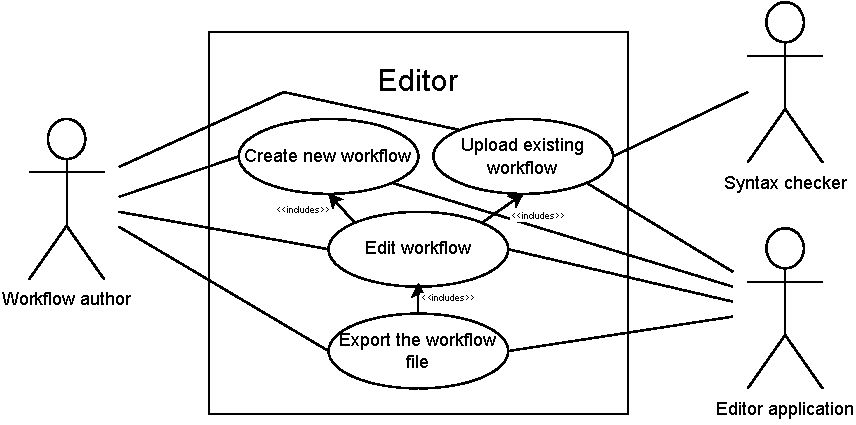
\includegraphics{./img/editorUC.pdf}
    \caption{Editor - Use Case UML diagram}
\end{figure}

% \begin{figure}[h!]
%     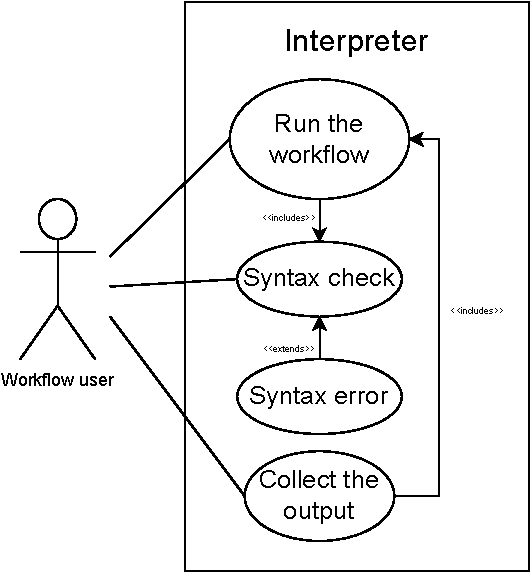
\includegraphics{./img/interpreterUC.pdf}
%     \caption{Interpreter - Use Case UML diagram}
% \end{figure}


\defcitealias{PPatch21}{PPatch21}
\defcitealias{PReadme22}{PReadme22}

\section*{Related Work}
As of now, there are already numerous solutions for automating web actions on the market. 
A majority of those uses existing web browsers and offer a programmable interface for simulating user input.

\textbf{Cypress} is a \ac{E2E} Javascript testing framework containing various assertions for \ac{QA} testing of webpages.
It supports multiple web browsers and offers its own UI and toolkit for test programming and running. 
Due to its strong orientation towards testing, it does not provide much methods for data extraction and crawling.

\textbf{Selenium WebDriver} is a fairly popular tool among web UI testers, as it offers a wide variety of methods for \ac{QA} testing.
Distributed as a multilanguage library, Selenium implements a high-level interface for controlling web browsers from code.
% Aside from regular commercial web browsers, Selenium also implements interfaces for PhantomJS and HTMLUnit, both headless scriptable browsers used as a lightweight alternative to regular browsers.

\textbf{Puppeteer} is a low-level library used for web browser automation. 
Unlike Cypress and Selenium, Puppeteer supports Chrome (or Chromium) as its only backend browser as of now (\today).

The communication with the browser is implemented via WebSockets and the DevTools Protocol, a Chromium-specific set of commands.
This allows Puppeteer to exceed Selenium both in stability and performance, sporting up to $17\%$ speedup in benchmarks \citepalias{Chck21}.

\textbf{Playwright} is another low-level library multilanguage library offering programmable ways of controlling web browser.
For browser communication, Playwright uses similiar technology as Puppeteer, unlike Puppeteer, Playwright supports multiple commercial browsers (Chromium, Firefox, Webkit as of \today).

Due to differences between browsers and partial incompatibility of protocols, Playwright is distributed with patched versions of Firefox and Webkit \citepalias{PPatch21}.
Stock versions of Chromium based browsers (Google Chrome, Microsoft Edge) are supported. \citepalias{PReadme22}

\vspace{\baselineskip}

All the aforementioned examples however require programming, which can mean a significant barrier to entry for beginners.


\chapter{Design}

This chapter describes decisions made while designing parts of the project. 
It contains separate sections for all three parts of the project, i.e. \textit{the format}, \textit{the interpreter} and \textit{the editor}.

Design decisions made here should reflect the requirements mentioned in the previous chapter.
These decisions also directly influence the implementation of the project described further.

\section{Workflow definition format}

As both the \textit{interpreter} and \textit{the editor} work directly with the files containing the workflow definitions, the first part of the project to be designed is the workflow definition format itself.

The workflow definition files should contain all the information needed to describe an arbitrary web-related workflow. 
The files in this format should also be parsable, human- and machine-readable and provide a simple yet powerful way of programming the web automations.

\subsection{Programming logic}

As the workflow definitions are computer programs of sorts, the first design decision needs to be what programming concepts will the file format implement.
To retain the steep learning curve and user-friendliness, this programming ``language'' also should not be too complicated.

The popularity of other automation tools shows that one of the simplest forms of programming is \textit{declarative programming}.
Defining the desired results rather than describing the complete control flow allows users to program the automations without being exposed to complicated programming principles.

Inspired by logic programming languages such as \textit{Prolog}, the workflow definition should contain a set of \textit{conditions} describing a possible state of the environment, connected to their respective \textit{reactions}, describing a sequence of actions to be carried out in case the condition applies.

% The similarity with \textit{Prolog} can be seen here, with the \textit{conditions} corresponding to \textit{Prolog's} fact \textit{heads} and \textit{reactions} to their respective \textit{bodies}.

\subsection{Conditions}

As stated before, the workflow definition format should allow the user to specify web environment-related conditions for running the automation steps.

Such conditions can be e.g. the browser visiting a certain \texttt{url}, the current page containing certain \texttt{selectors} or the current browser session having \texttt{cookies} set to specific values.

Moreover, the format should allow the user to combine the base conditions using \textit{boolean operators} to create more comprehensible and compact syntax.

Following through with the \textit{Prolog} comparison, the workflow definition could look something like this:

\begin{minipage}{0.95\linewidth}
\begin{verbatim}
    % X is denoting the current state of the browser
    % Y is to be unified with the next state

    nextState(X, Y) :- url(X, "https://jindrich.bar"),
                        % action to be 
                        % executed on 
                        % https://jindrich.bar
    
    nextState(X, Y) :- selector(X, "button"),
                        % action to be 
                        % executed if the current 
                        % page contains a button
    
    nextState(X, Y) :- cookies(X, "key", "value"),
                        % action to be 
                        % executed if the current 
                        % browser session has the
                        % `key` cookie for the  
                        % page set to `value`
    
    nextState(X, Y) :- url(X, "https://example.org"),
                       selector(X, "input"),
                        % action to be 
                        % executed in case of both
                        % conditions matching 
                        % (boolean AND example)

\end{verbatim}
\end{minipage}

The conditions might also provide support for advanced techniques, such as wildcards or regular expressions.
Those would be particularly useful for the URLs e.g. for targetting a specific domain, TLD etc.

\subsection{Reactions}

The workflow definition format should also allow the user to specify the actions to be carried out when the respective condition matches.

Those can be e.g. \texttt{click}, \texttt{goto}, \texttt{scrapeData} and similar. 
The actions should be chainable, allowing the user to specify a set of actions to be executed sequentially, without additional condition matching between those.

Completing the \textit{Prolog-inspired} example from the previous section, the complete workflow definition would look like this:

\begin{minipage}{0.95\linewidth}
\begin{verbatim}
    % X is denoting the current state of the browser
    % Y is to be unified with the next state

    nextState(X, Y) :- url(X, "https://jindrich.bar"),
                       goto(X, Y, "https://example.org").
    
    nextState(X, Y) :- selector(X, "button"),
                       click(X, Y, "button").
    
    nextState(X, Y) :- cookies(X, "key", "value"),
                       click(X, Y, "logout").
    
    nextState(X, Y) :- url(X, "https://example.org"),
                       selector(X, "input"),
                       fill(X, "input", "hello").

\end{verbatim}
\end{minipage}

The mock implementation of the workflow definition file in \textit{SWI-Prolog} is available as a \href{https://swish.swi-prolog.org/p/dwaim.pl}{snippet}\footnote{Available at \url{https://swish.swi-prolog.org/p/dwaim.pl}} in the \textit{Prolog} online execution environment \textit{Swish}. 

Please note that in this case, the \textit{Prolog} interpreter is actually taking role of the workflow interpreter.

\multilinebox{
    \smallskip
    \textbf{Note:} This example also shows that the new state of the browser depends only on the preceding one. 
    
    Such quality, also called \textit{memorylessness}, or \textit{Markov property}, simplifies both the interpreter design and the programming concept itself.
    It might also allow for some optimizations utilizing parallel execution. 
    \smallskip
}

\subsection{Serialization}

\defcitealias{GTrends22}{GTrends22}
\defcitealias{Medium21}{Medium21}

Finally, the workflow definition needs to be physically stored in a file. 
As it would be rather counterproductive to develop a custom file format for storing the conditions and reactions, the workflow definitions might be stored using a host meta-format.

Based on the hierarchical nature of both \textit{condition-action} pairs and possibly recursive nature of the \textit{conditions} themselves, it would be only logical to store the definitions using a hierarchical data format like \textit{JSON}, \textit{XML} or \textit{YAML}.

Comparing these formats, \textit{JSON} comes out as the most popular \citepalias{GTrends22} and most space-saving \citepalias{Medium21}. 
While the advanced features of \textit{XML} are invaluable when working with complex structured data, it is perhaps too complicated for storing well-defined workflow definitions.

With YAML taking first place, JSON is also a runner-up in human readability.
While improving the file legibility, the indentation oriented nature of YAML makes it very prone to input errors - this problem is absent in JSON because of its bracket-oriented grammar.

For the reasons mentioned, the workflow definition format will be built upon JSON - a host format providing a simple, human-readable serialization for structured schema of the definitions.

\subsubsection{}

\chapter*{Conclusion}
\addcontentsline{toc}{chapter}{Conclusion}


%%% Bibliography
%%% Bibliography (literature used as a source)
%%%
%%% We employ bibTeX to construct the bibliography. It processes
%%% citations in the text (e.g., the \cite{...} macro) and looks up
%%% relevant entries in the bibliography.bib file.
%%%
%%% The \bibliographystyle command selects, which style will be used
%%% for references from the text. The argument in curly brackets is
%%% the name of the corresponding style file (*.bst). Both styles
%%% mentioned in this template are included in LaTeX distributions.

\bibliographystyle{plainnat}    %% Author (year)
% \bibliographystyle{unsrt}     %% [number]

\renewcommand{\bibname}{Bibliography}

%%% Generate the bibliography. Beware that if you cited no works,
%%% the empty list will be omitted completely.

\bibliography{bibliography}

%%% If case you prefer to write the bibliography manually (without bibTeX),
%%% you can use the following. Please follow the ISO 690 standard and
%%% citation conventions of your field of research.

% \begin{thebibliography}{99}
%
% \bibitem{lamport94}
%   {\sc Lamport,} Leslie.
%   \emph{\LaTeX: A Document Preparation System}.
%   2nd edition.
%   Massachusetts: Addison Wesley, 1994.
%   ISBN 0-201-52983-1.
%
% \end{thebibliography}


%%% Figures used in the thesis (consider if this is needed)
\listoffigures

%%% Tables used in the thesis (consider if this is needed)
%%% In mathematical theses, it could be better to move the list of tables to the beginning of the thesis.
\listoftables

%%% Abbreviations used in the thesis, if any, including their explanation
%%% In mathematical theses, it could be better to move the list of abbreviations to the beginning of the thesis.

\chapwithtoc{List of Abbreviations}

\begin{acronym}
 \acro{GUI}{graphical user interface}
 \acro{API}{application programming interface}
 \acro{CLI}{command line interface}
 \acro{RPA}{robotic process automation}
 \acro{QA}{quality assurance}
 \acro{E2E}{end-to-end}
 \acro{SW}{software}
 \acro{UX}{user experience}
 \acro{UI}{user interface}
 \acro{CDP}{Chrome DevTools Protocol}
 \acro{IDE}{integrated development environment}
 \acro{JS}{JavaScript}
 \acro{TS}{TypeScript}
 \acro{JSX}{JavaScript Extended Syntax}
 \acro{HTML}{Hypertext Markup Language}
 \acro{WYSIWYG}{\href{https://en.wiktionary.org/wiki/WYSIWYG}{What You See Is What You Get}}
 \acro{DOM}{Document Object Model}
 \acro{CORS}{cross-origin resource sharing}
 \acro{NPM}{\href{https://www.npmjs.com/}{Node Package Manager}}
 \acro{SUS}{Software Usability Scale}
\end{acronym}

%%% Attachments to the bachelor thesis, if any. Each attachment must be
%%% referred to at least once from the text of the thesis. Attachments
%%% are numbered.
%%%
%%% The printed version should preferably contain attachments, which can be
%%% read (additional tables and charts, supplementary text, examples of
%%% program output, etc.). The electronic version is more suited for attachments
%%% which will likely be used in an electronic form rather than read (program
%%% source code, data files, interactive charts, etc.). Electronic attachments
%%% should be uploaded to SIS and optionally also included in the thesis on a~CD/DVD.
%%% Allowed file formats are specified in a provision of the rector no. 72/2017.
\unless\ifdefined\short
	\appendix
	\chapter{Attachments}

	\section{First Attachment}

\fi
\openright
\end{document}
